
\section{Mutation}

\begin{frame}{Intended Learning Outcomes}

	\underline{Mutation}

	\bigskip

	In this lecture you will learn
  	\begin{itemize}
                \item to appreciate the effects of novel mutations on allele frequencies
                \item to describe the concepts of mutation and substitution rate
                \item to calculate divergence times using the molecular clock from genomic data with \texttt{R}
        \end{itemize}

\end{frame}

\begin{frame}{Mutations}

        New mutations arise to produce new genetic variation that genetic drift can act on:
        \begin{itemize}
                \item deletions
                \item insertions
                \item translocations
                \item point mutations
        \end{itemize}

        Any of these mutations can be represented with a di-allelic model (e.g. presence/absence)
        if we assume that multiple mutations cannot occur in the same location*.

	\bigskip
        \tiny * more on this later

\end{frame}


\begin{frame}{Effect of mutations on allele frequency}

	\bigskip

	Assume that the $a$ allele in each individual randomly mutates to $A$ with probability $\mu$ 
	(\textbf{mutation rate}) in each generation.

	\begin{figure}
                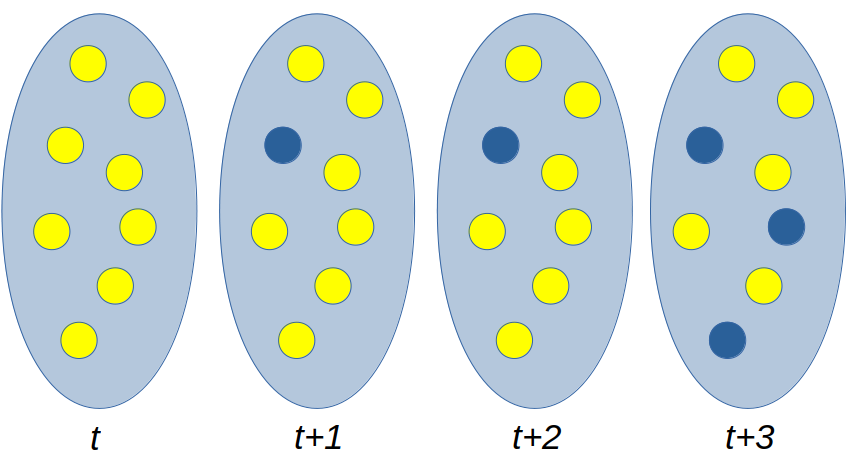
\includegraphics[width=0.8\textwidth]{Pics/mutation}
        \end{figure}


\end{frame}

\begin{frame}{Effect of mutations on allele frequency}

        \begin{figure}
                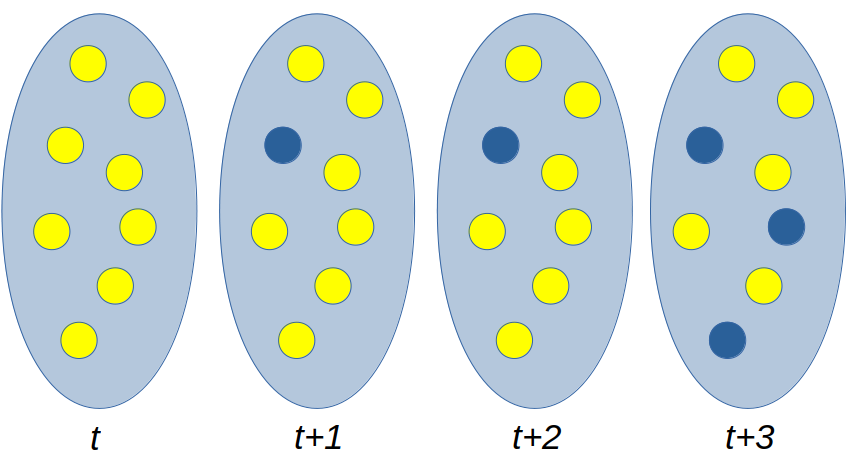
\includegraphics[width=0.6\textwidth]{Pics/mutation}
        \end{figure}

	What is the $E[f_A(t+1)]$ given $f_A(t)$ and $\mu$?
	\pause
	\begin{equation}
		E[f_A(t+1)] = f_A(t) + \mu f_a(t)
	\end{equation}

	\tiny{jupyter-notebook: mutation}

\end{frame}


\begin{frame}{Effect of mutations on allele frequency}

	If mutations occur in both directions, e.g. mutations occur at rate $\mu_{a \rightarrow A}$ from $a$
	to $A$ and $\mu_{A \rightarrow a}$ from $A$ to $a$, then
	\begin{equation}
		E[f_A(t+1)] = (1 - \mu_{A \rightarrow a} ) f_A(t) + \mu_{a \rightarrow A} f_a(t)
	\end{equation}

	\bigskip
	\tiny{jupyter-notebook: mutation}

\end{frame}


\begin{frame}{Effect of mutations on allele frequency}

	In the absence of other forces (e.g. genetic drift and selection), an equilibrium will
	eventually be established:
	\begin{equation}
		f_A = \frac{\mu_{a \rightarrow A}}{\mu_{a \rightarrow A}+\mu_{A \rightarrow a}}
	\end{equation}

\end{frame}


\begin{frame}{Mutation rate}

	\begin{figure}
                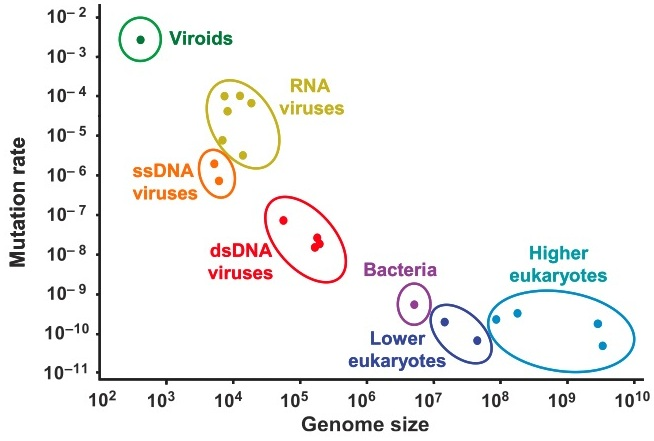
\includegraphics[width=0.5\textwidth]{Pics/mutrate}
        \end{figure}

	\small
	\begin{itemize}
		\item mutation is a weak force in higher organisms
		\item with no genetic drift, it takes a long time for the allele frequency to reach equilibrium
		\item we can often ignore recurrent mutations
	\end{itemize}

\end{frame}


\begin{frame}{Probability of fixation}

	The probability that an allele of frequency $1/(2N)$ goes to fixation is $1/(2N)$.

	\bigskip

	\pause
	$Pr(\texttt{fixation of allele A}) = N_A \times (1/2N) = f_A(t) $ at generation $t$.

	\begin{block}{}
	In the absence of selection and mutation, the probability of fixation of an allele is simply its allele frequency.
	It does not depend on the population size.
	\end{block}

\end{frame}


\begin{frame}{Rate of substitution}

	\small
	\begin{block}
	Rate at which mutations accumulate \textbf{between species}. 
	Substitution refers to mutations that have gone to fixation. 
	\end{block}

	\vskip 0.3cm

	Assume:
	\begin{itemize}
		\item mutation rate $\mu$: in each generation $\mu$ new mutations occur in each gene copy (e.g. per site, per gene, ...)
		\item $2N$ gene copies
	\end{itemize}

	\pause

	The expected number of mutations each generation that eventually will go to fixation is
	\begin{equation*}
		2N\mu \times 1/(2N) = \mu
	\end{equation*}
	The rate of substituion is simply the mutation rate.

\end{frame}


\begin{frame}{Molecular clock}

	If
	\begin{itemize}
		\item no selection
		\item "low" mutation rate (not affecting allele frequencies much)
		\item constant mutation rate
	\end{itemize}
	then the rate of substitution should be contant \textit{in time}.

	\bigskip

	\begin{block}{}
		Mutations can be used to date divergence between species.
	\end{block}
	How?

\end{frame}


\begin{frame}{Molecular clock}

	\begin{columns}

        	\column{0.5\textwidth}

                \begin{figure}
                        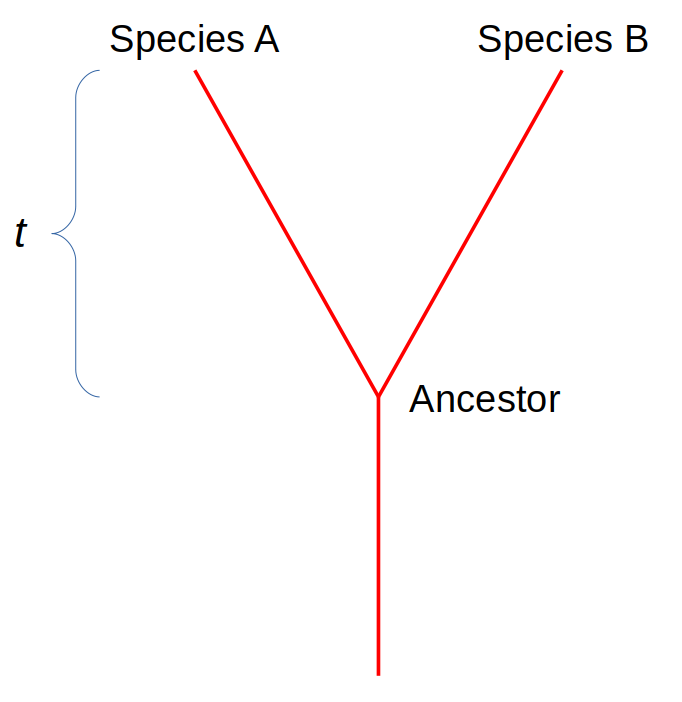
\includegraphics[width=0.9\textwidth]{Pics/divergence}
                \end{figure}

                \column{0.5\textwidth}
		\small
		The expected number of nucleotide differences separating sequences of the same genes in the two species is $E[d_{AB}] = 2 \mu t_{AB}$.
		
		\bigskip

		Therefore
		\begin{itemize}
			\item $t_{AB}=\frac{2\mu}{d_{AB}}$ or
			\item $\mu = \frac{d_{AB}}{2t_{AB}}$
		\end{itemize}

        \end{columns}

\end{frame}


\begin{frame}{Molecular clock}

	Caveats:
	\begin{itemize}
		\item it depends on an estimate of $\mu$
		\item it assumes no natural selection acting
		\item it assumes that mutation rate is constant and equal among different species
	\end{itemize}

	\bigskip
	Not very realistic but a good approximate for closely related species.

\end{frame}


\begin{frame}{Dating human-chimpanzee divergence time}

	\begin{figure}
        	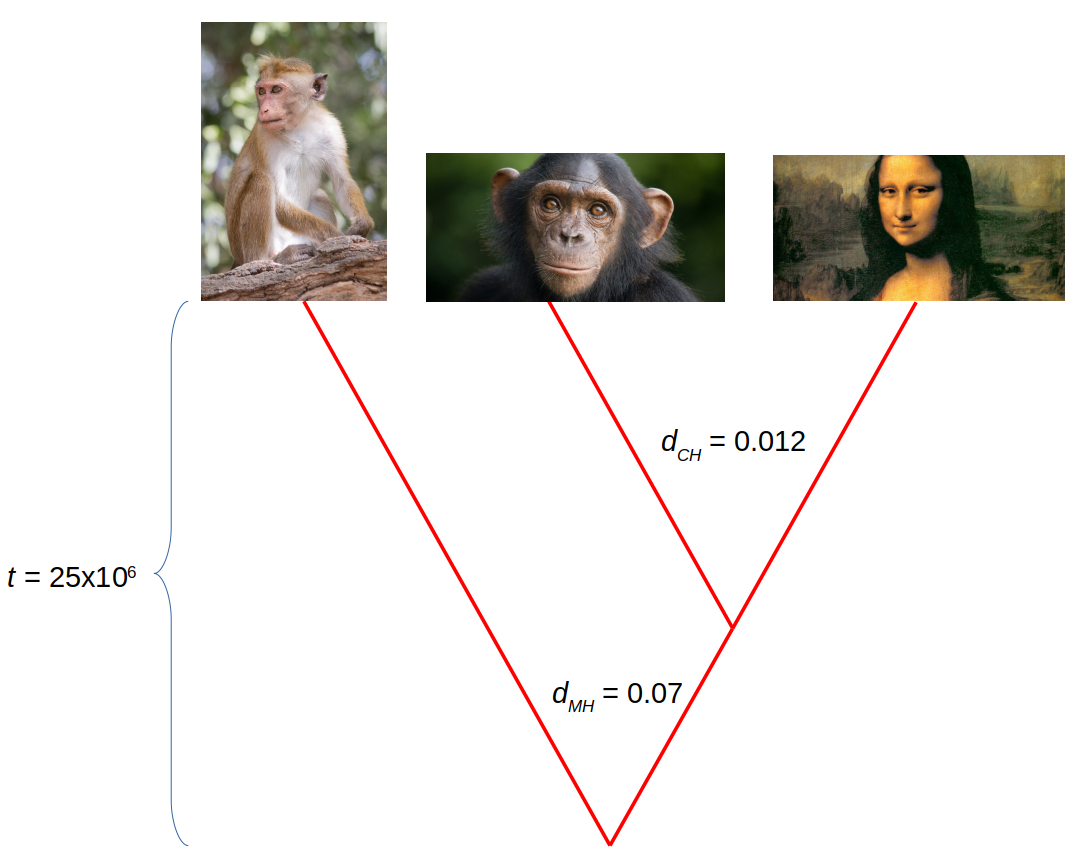
\includegraphics[width=0.75\textwidth]{Pics/dating}
        \end{figure}

\end{frame}


\begin{frame}{Dating human-chimpanzee divergence time}

	$\mu = 0.07 / (2 \times 25 \times 10^6) = 1.4 \times 10^{-9}$ per site per year

	\bigskip

	$t = 0.012 / (2 \times 1.4 \times 10^{-9}) = 4.3$ million years ago

	\bigskip

	\small

	Compatible but shorted than expected: \\
	generation time as changed and therefore the rate per year changed \\
	effect of natural selection \\
	change in mutation rate \\
	errors in estimating nucleotidic divergence \\
	error in estimating human-macaque divergence time \\
	...
	
\end{frame}


\begin{frame}{Intended Learning Outcomes}

        \underline{Mutation}

	\bigskip

        In this lecture you have learnt
        \begin{itemize}
                \item to appreciate the effects of novel mutations on allele frequencies
                \item to describe the concepts of mutation and substitution rate
                \item to calculate divergence times using the molecular clock from genomic data with \texttt{R}
        \end{itemize}

\end{frame}


